\raggedbottom

%%%%%%%%%%%%%%%%%%%%%%%%%%%%%%%%%%%%%%%%%%%%%%%%%%%%%%%%%%%%%%%%%%%%%%%%%%%%%%%
% 4 DISEÑO Y DESARROLLO TÉCNICO MECATRÓNICO
%%%%%%%%%%%%%%%%%%%%%%%%%%%%%%%%%%%%%%%%%%%%%%%%%%%%%%%%%%%%%%%%%%%%%%%%%%%%%%%

% Título en \parbox: el estilo de capítulo no corta líneas largas.
\chapter[Diseño y desarrollo técnico mecatrónico]{\parbox[t]{0.72\textwidth}{\raggedright Diseño y desarrollo técnico mecatrónico}}
\label{cap:diseno_tecnico}

% PENDIENTE: texto introductorio del capítulo.

% La Contextualización se numera 4.0 según THESIS_STRUCTURE.md ([R][A]);
% su ubicación está por confirmar con el docente.
\setcounter{section}{-1}

%%%%%%%%%%%%%%%%%%%%%%%%%%%%%%%%%%%%%%%%%%%%%%%%%%%%%%%%%%%%%%%%%%%%%%%%%%%%%%%
% 4.0 CONTEXTUALIZACIÓN DEL SISTEMA ACTUAL (antes «Antecedentes del Problema»)
%%%%%%%%%%%%%%%%%%%%%%%%%%%%%%%%%%%%%%%%%%%%%%%%%%%%%%%%%%%%%%%%%%%%%%%%%%%%%%%

\section{Contextualización del sistema actual}
\label{subsec:antecedentes_problema}
\label{sec:contextualizacion}

% PENDIENTE: completar con proporciones de receta, características de la harina
% (tamaño de grano, densidad) y máquinas existentes; requieren fuente o relevamiento.

El levantamiento de campo en la Panadería San Miguel se concentró en el
procedimiento manual de dosificación de harina. El intervalo analizado
comprendió desde la preparación del recipiente receptor para el pesaje
hasta la devolución del recipiente de transporte a la zona de
almacenamiento. El abastecimiento y la apertura de las bolsas de harina,
el traslado hacia la amasadora y las operaciones de elaboración siguientes
quedaron fuera del registro temporal.

La Figura~\ref{fig:dfd_dosificacion} presenta la secuencia del procedimiento
manual registrado. El diagrama comprende la preparación del recipiente,
el uso de la función TARE\footnote{TARE: función de la balanza utilizada
para compensar la masa del recipiente y establecer la indicación de cero
antes de incorporar la harina.}, la incorporación de harina, la medición
de la cantidad acumulada y su comparación con la cantidad objetivo. Cuando la cantidad registrada es
inferior a la cantidad objetivo, se incorpora harina adicional. El bloque
final comprende la comprobación de la lectura final y la devolución del
recipiente de transporte.

\begin{figure}[H]
    \centering
    \resizebox{0.6\textwidth}{!}{%
        {\setlength{\fboxsep}{14pt}
        \fbox{\begin{tikzpicture}[
    >=Latex,
    node distance=0.45cm and 2.0cm,
    font=\small,
    proceso/.style={
        rectangle,
        draw,
        rounded corners=2pt,
        minimum width=4.6cm,
        minimum height=0.8cm,
        text width=4.0cm,
        align=center,
        inner ysep=3pt
    },
    decision/.style={
        diamond,
        draw,
        aspect=2.5,
        text width=3.6cm,
        align=center,
        inner sep=1.2pt
    },
    iniciofin/.style={
        rectangle,
        draw,
        rounded corners=12pt,
        minimum width=2.6cm,
        minimum height=0.65cm,
        align=center,
        inner ysep=2pt
    },
    flecha/.style={
        -{Latex[width=7pt,length=6pt]},
        thick
    }
]

% Flujo principal
\node[iniciofin] (inicio) {Inicio};

\node[proceso, below=of inicio] (preparar)
{Preparar recipiente Receptor};

\node[proceso, below=of preparar] (tara)
{Tarar balanza};

\node[proceso, below=of tara] (trasladar)
{Trasladar harina\\al recipiente receptor};

\node[proceso, below=of trasladar] (medir)
{Medir cantidad};

\node[decision, below=0.55cm of medir] (decision)
{¿Cantidad objetivo\\alcanzada?};

\node[proceso, below=0.55cm of decision] (finalizar)
{Finalizar dosificación};

\node[iniciofin, below=of finalizar] (fin)
{Fin};

% Bucle lateral
\node[
    proceso,
    left=1.4cm of decision,
    text width=2.2cm,
    minimum width=2.5cm
] (agregar)
{Agregar harina};

% Conexiones
\draw[flecha] (inicio) -- (preparar);
\draw[flecha] (preparar) -- (tara);
\draw[flecha] (tara) -- (trasladar);
\draw[flecha] (trasladar) -- (medir);
\draw[flecha] (medir) -- (decision);

\draw[flecha]
    (decision.south)
    -- node[right,font=\small] {Sí}
    (finalizar.north);

\draw[flecha] (finalizar) -- (fin);

\draw[flecha]
    (decision.west)
    -- ++(-1.0,0)
    node[above,font=\small,pos=0.35] {No}
    -- (agregar.east);

\draw[flecha]
    (agregar.north)
    |- (medir.west);

\end{tikzpicture}
}}%
    }
    \caption{Diagrama de flujo del procedimiento manual de dosificación de harina.}
    \label{fig:dfd_dosificacion}
    \vspace{0.2em}
    {\footnotesize Fuente: Elaboración propia.}
\end{figure}

El operario inició el procedimiento colocando el recipiente receptor sobre
la balanza. A continuación, utilizó la función TARE y comprobó la indicación de cero. Esta lectura estableció la referencia
inicial para registrar la cantidad de harina incorporada.

Desde el punto de pesaje, el operario se desplazó hacia la zona de
almacenamiento, recogió una carga de harina con el recipiente de transporte
y retornó a la balanza. Luego descargó la harina en el recipiente receptor.
Después de cada descarga, la balanza indicó la cantidad acumulada de harina.

La Figura~\ref{fig:balanza_recipiente} (a) muestra el recipiente utilizado
para recoger y trasladar la harina, mientras que la
Figura~\ref{fig:balanza_recipiente} (b) muestra el recipiente receptor
colocado sobre la balanza durante la dosificación.

\begin{figure}[H]
    \setstretch{1}
    \captionsetup{skip=4pt}
    \centering

    \begin{minipage}[t]{0.48\textwidth}
        \vspace{0pt}
        \centering
        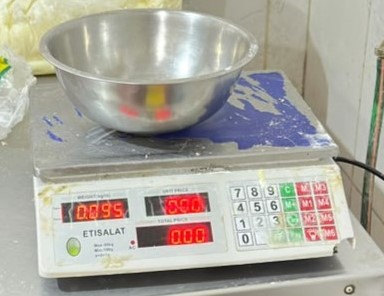
\includegraphics[
            width=\linewidth,
            height=5.2cm,
            keepaspectratio
        ]{images/marcoref/recipiente_transporte.jpg}

        \smallskip
        {\small (a) Recipiente de transporte.}
    \end{minipage}
    \hfill
    \begin{minipage}[t]{0.48\textwidth}
        \vspace{0pt}
        \centering
        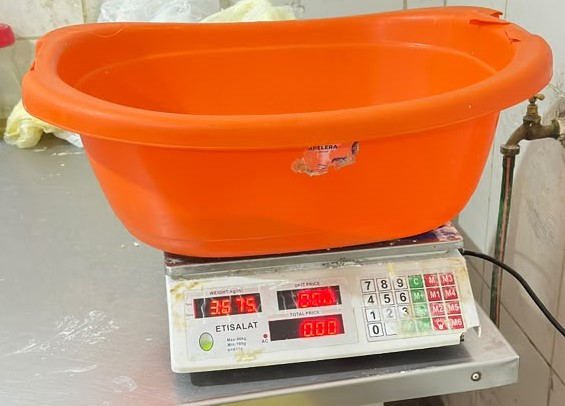
\includegraphics[
            width=\linewidth,
            height=5.2cm,
            keepaspectratio
        ]{images/marcoref/balanza_recipiente_vacio.jpg}

        \smallskip
        {\small (b) Recipiente receptor sobre la balanza.}
    \end{minipage}

    \caption{Recipientes utilizados durante la dosificación manual de harina.}
    \label{fig:balanza_recipiente}
    \vspace{0.2em}
    {\footnotesize Fuente: Registro fotográfico propio.}
\end{figure}

La incorporación de harina se desarrolló entre la zona de almacenamiento
y el punto de pesaje. La Figura~\ref{fig:croquis_panaderia} muestra la
ubicación de estos sectores dentro del área de trabajo. Las cotas de
$3{,}20\ \mathrm{m}$ y $0{,}90\ \mathrm{m}$ corresponden a tramos medidos
en planta relacionados con los desplazamientos realizados durante la
dosificación. Estas referencias caracterizan la separación física entre
el almacenamiento de harina y el punto de pesaje.

\begin{figure}[H]
    \centering
    \resizebox{0.9\textwidth}{!}{%
        % Planta esquemática: las coordenadas gráficas no representan una escala.
% El acceso y el giro de la puerta corresponden a la disposición indicada por el estudiante.
\begin{tikzpicture}[
    font=\small,
    equipo/.style={draw, line width=0.6pt, align=center, inner sep=5pt},
    relevante/.style={equipo, fill=black!5},
    cota/.style={thin, {Latex[length=4pt]}-{Latex[length=4pt]}},
    guia/.style={thin, densely dashed, black!60}
]
% Límite del área y abertura del acceso.
\draw[line width=0.8pt] (9,0) -- (0,0) -- (0,7) -- (14,7)
    -- (14,0) -- (10.3,0);
\draw[line width=0.6pt] (9,0) -- (9,1.3);
\draw[thin, dashed] (10.3,0) arc[start angle=0,end angle=90,radius=1.3];
\node[align=center, anchor=north] at (9.65,-0.18)
    {Acceso al área de trabajo};

% Equipos y superficies, en la disposición relativa del croquis original.
\node[equipo, minimum width=2cm, minimum height=2.1cm,
    text width=1.8cm, font=\footnotesize] at (1.3,5.65) {Almacén de\\ingredientes};
\node[equipo, minimum width=4.45cm, minimum height=1.5cm,
    text width=4cm] at (5.05,5.95) {Mesa de laminado\\y formado};
\node[relevante, minimum width=2.85cm, minimum height=1.6cm,
    text width=2.5cm] (harina) at (9.35,5.95) {Almacenamiento\\de harina};
\node[relevante, minimum width=2.25cm, minimum height=1.5cm,
    text width=1.85cm] at (12.55,5.95) {Amasadora};
\node[equipo, minimum width=4.8cm, minimum height=2.25cm,
    text width=4.25cm] at (6.15,3) {Mesa de reposo\\y porcionado};
\node[equipo, minimum width=1.6cm, minimum height=1.1cm,
    text width=1.25cm, font=\footnotesize, anchor=south] at (8,0.2) {Divisora\\de masa};

% La balanza se identifica dentro de la mesa vinculada a la dosificación.
\draw[fill=black!5, line width=0.6pt] (11.4,0.2) rectangle (13.7,4.6 );
\node[align=center, text width=2.05cm, font=\footnotesize] at (12.55,3.0)
    {Mesa de\\ingredientes y\\dosificación};
\node[equipo, fill=white, text width=1.65cm,
    minimum height=0.95cm, font=\footnotesize] (balanza) at (12.55,1.1)
    {Balanza\\Punto de pesaje};

% Cotas transcritas
\draw[guia] (10.2,5.15) -- (10.65,5.15);
\draw[guia] (10.2,1.1) -- (11.4,1.1);
\draw[cota] (10.3,1.1) -- node[left, fill=white, inner sep=2pt]
    {3,20 m} (10.3,5.15);
\draw[cota] (10.3,0.75) -- node[below, fill=white, inner sep=1pt,
    font=\footnotesize] {0,90 m} (11.4,0.75);
\draw[guia] (14,0) -- (14.7,0);
\draw[guia] (14,7) -- (14.7,7);
\draw[cota] (14.55,0) -- (14.55,7);
\node[rotate=90, anchor=north, inner sep=0pt] at (14.75,3.5) {4,10 m};

\end{tikzpicture}
%
    }
    \caption{Distribución de las zonas de trabajo de la Panadería San Miguel.}
    \label{fig:croquis_panaderia}
    \vspace{0.2em}
    {\footnotesize Fuente: Elaboración propia.}
\end{figure}

La Figura~\ref{fig:entorno_pesaje} (a) muestra la zona de almacenamiento
de harina y la Figura~\ref{fig:entorno_pesaje} (b) la mesa de ingredientes
donde se ubica el punto de pesaje. Ambos registros corresponden a los
sectores vinculados por los desplazamientos realizados durante la
dosificación.

\begin{figure}[H]
    \centering

    \begin{minipage}[t]{0.48\textwidth}
        \vspace{0pt}
        \centering
        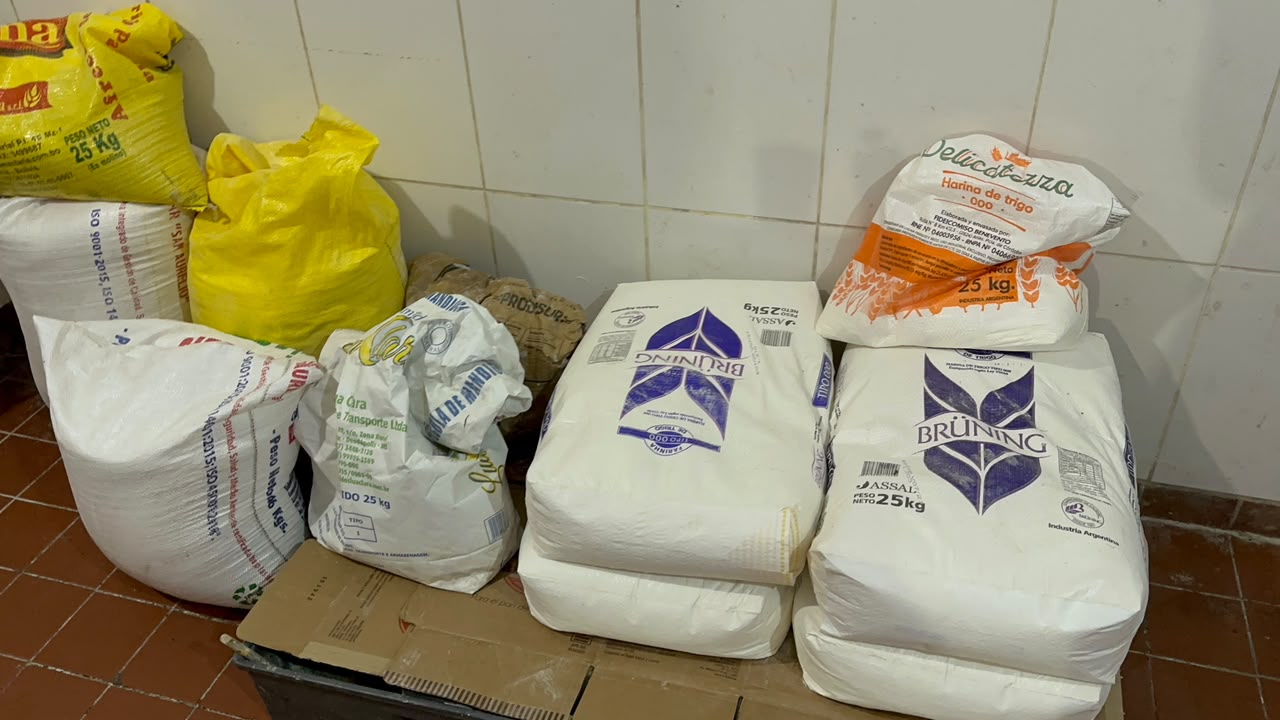
\includegraphics[
            width=\linewidth,
            height=4.3cm,
            keepaspectratio
        ]{images/marcoref/ubicacion_bolsas_harina.jpg}

        \smallskip
        {\small (a) Almacenamiento de harina.}
    \end{minipage}
    \hfill
    \begin{minipage}[t]{0.51\textwidth}
        \vspace{0pt}
        \centering
        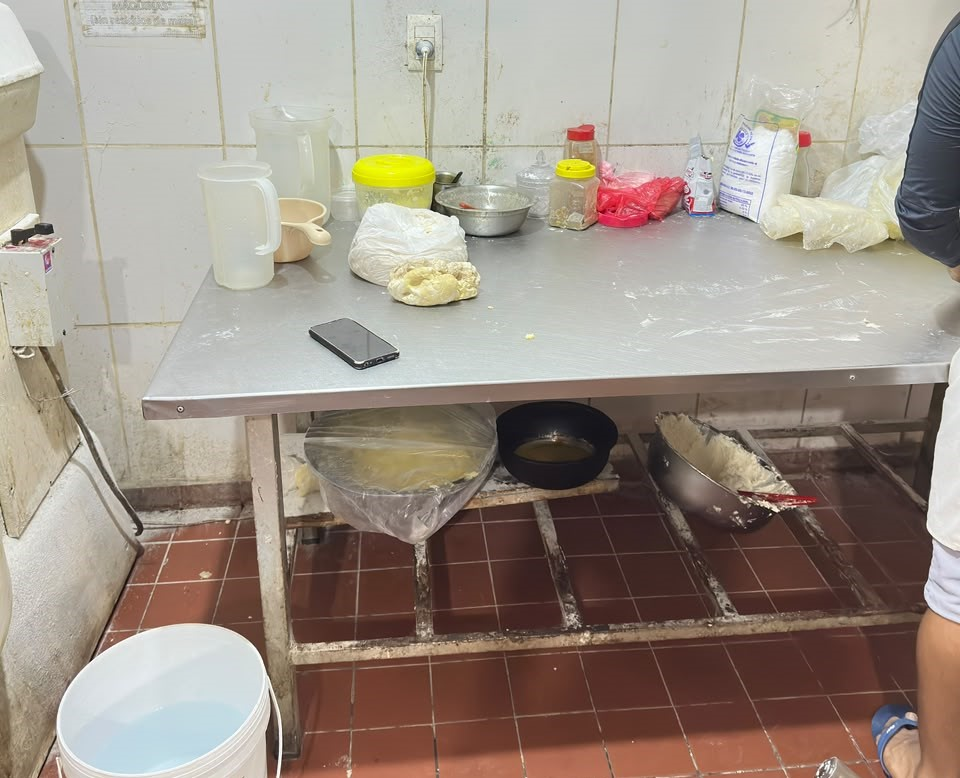
\includegraphics[
            width=\linewidth,
            height=4.3cm,
            keepaspectratio
        ]{images/marcoref/mesa_ingredientes_balanza.jpg}

        \smallskip
        {\small (b) Mesa de ingredientes y punto de pesaje.}
    \end{minipage}

    \caption{Área de trabajo relacionada con la dosificación de harina.}
    \label{fig:entorno_pesaje}
    \vspace{0.2em}
    {\footnotesize Fuente: Registro fotográfico propio.}
\end{figure}

Con cada carga principal, el operario comparó la cantidad acumulada con la
cantidad objetivo de la preparación. Cuando la lectura permaneció por
debajo de dicha cantidad, el operario retornó a la zona de almacenamiento
y repitió las operaciones de recogida, traslado y descarga. Esta secuencia
continuó hasta completar las tres o cuatro cargas principales registradas
en cada ciclo.

El ajuste final se realizó con la harina remanente en el recipiente de
transporte, sin un nuevo desplazamiento hacia la zona de almacenamiento.
El operario incorporó la cantidad restante, comprobó la lectura final de
la balanza y devolvió el recipiente de transporte. Esta devolución marcó
el cierre del intervalo analizado.

La Figura~\ref{fig:ajuste_final_harina} (a) muestra el ajuste final realizado
por el operario y la Figura~\ref{fig:ajuste_final_harina}(b) el recipiente
receptor con la harina dosificada sobre la balanza. Ambos registros
corresponden a la etapa final del procedimiento.

\begin{figure}[H]
    \setstretch{1}
    \captionsetup{skip=4pt}
    \centering

    \begin{minipage}[t]{0.48\textwidth}
        \vspace{0pt}
        \centering
        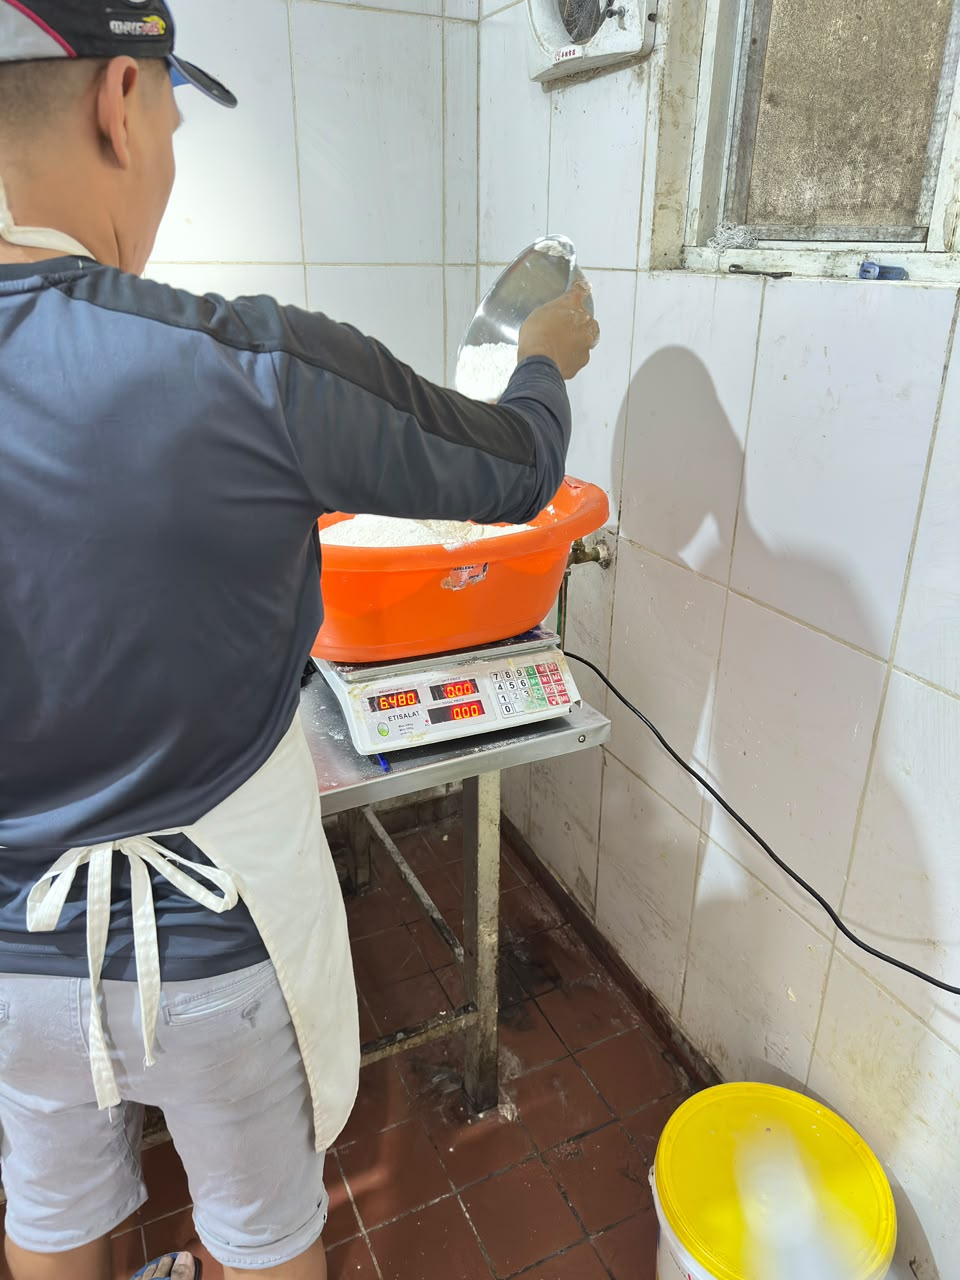
\includegraphics[
            width=\linewidth,
            height=5.2cm,
            keepaspectratio
        ]{images/marcoref/ajuste_final_operario.jpg}

        \smallskip
        {\small (a) Ajuste final realizado por el operario.}
    \end{minipage}
    \hfill
    \begin{minipage}[t]{0.48\textwidth}
        \vspace{0pt}
        \centering
        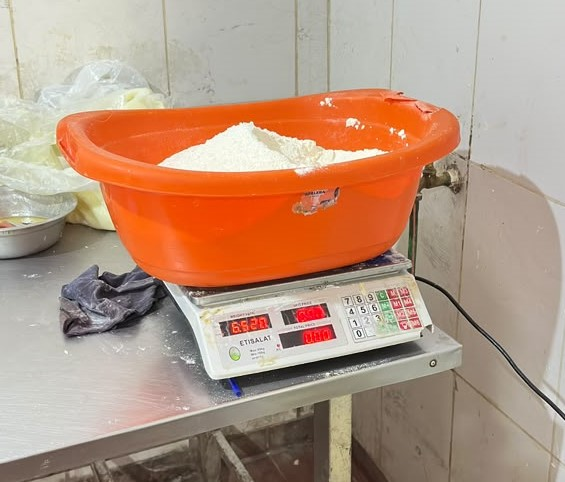
\includegraphics[
            width=\linewidth,
            height=5.2cm,
            keepaspectratio
        ]{images/marcoref/harina_dosificada.jpg}

        \smallskip
        {\small (b) Recipiente receptor con harina dosificada.}
    \end{minipage}

    \caption{Ajuste final y harina dosificada sobre la balanza.}
    \label{fig:ajuste_final_harina}
    \vspace{0.2em}
    {\footnotesize Fuente: Registro fotográfico propio.}
\end{figure}

%%%%%%%%%%%%%%%%%%%%%%%%%%%%%%%%%%%%%%%%%%%%%%%%%%%%%%%%%%%%%%%%%%%%%%%%%%%%%%%
% COBERTURA Y RESULTADOS DEL LEVANTAMIENTO
%%%%%%%%%%%%%%%%%%%%%%%%%%%%%%%%%%%%%%%%%%%%%%%%%%%%%%%%%%%%%%%%%%%%%%%%%%%%%%%

Se registraron cinco ciclos de dosificación el 2 de septiembre de 2026
y dos el 5 de septiembre. En cada ciclo se registraron la cantidad objetivo
y la cantidad final indicada por la balanza. Además, se midió el tiempo
desde la preparación del recipiente y el uso de la función TARE hasta la
devolución del recipiente de transporte, incluidas las cargas, los
desplazamientos y el ajuste final. La diferencia de harina corresponde
a la cantidad final menos la cantidad objetivo.

La Tabla~\ref{tab:resumen_dosificacion} resume los resultados de los ciclos
registrados en cada jornada observada. Para cada jornada se presentan el
número de ciclos, la cantidad objetivo acumulada de harina, la cantidad
final indicada por la balanza, la diferencia entre ambas cantidades y el
tiempo total registrado. El detalle de los registros
se encuentra en los Apéndices~\ref{ap:registros_campo} y
\ref{ap:tablas_dosificacion}.

\begin{table}[H]
    \centering
    \caption{Resultados consolidados de los ciclos de dosificación manual
    registrados en cada jornada observada.}
    \label{tab:resumen_dosificacion}
    \footnotesize
    \setstretch{1}

    \setlength{\tabcolsep}{3pt}
    \renewcommand{\arraystretch}{1.35}

    \begin{tabular}{lccccc}
        \toprule[1pt]

        \textbf{\shortstack{Jornada\\observada}} &
        \textbf{\shortstack{Ciclos\\registrados}} &
        \textbf{\shortstack{Harina objetivo\\(kg)}} &
        \textbf{\shortstack{Harina final\\(kg)}} &
        \textbf{\shortstack{Diferencia\\(kg)}} &
        \textbf{\shortstack{Tiempo total\\(s)}} \\
        \midrule[1pt]

        \shortstack{Ordinaria\\02/09/2026} &
        5 &
        $36{,}500$ &
        $36{,}578$ &
        $+0{,}078$ &
        $304{,}5$ \\
        \midrule[1pt]

        \shortstack{Sábado\\05/09/2026} &
        2 &
        $11{,}500$ &
        $11{,}565$ &
        $+0{,}065$ &
        $107{,}4$ \\
        \midrule[1pt]

        \textbf{Total de la muestra} &
        \textbf{7} &
        $\mathbf{48{,}000}$ &
        $\mathbf{48{,}143}$ &
        $\mathbf{+0{,}143}$ &
        $\mathbf{411{,}9}$ \\
        \bottomrule[1pt]
    \end{tabular}

    \vspace{0.5em}

    {\footnotesize
    Fuente: Elaboración propia.}
\end{table}

En la jornada ordinaria se registraron cinco ciclos, con un tiempo
acumulado de $304{,}5\ \mathrm{s}$. En la jornada de sábado se registraron
dos ciclos, que acumularon $107{,}4\ \mathrm{s}$. En conjunto, los siete
ciclos observados sumaron $411{,}9\ \mathrm{s}$.

En cuanto a la cantidad de harina, los siete ciclos acumularon
$48{,}000\ \mathrm{kg}$ como cantidad objetivo y
$48{,}143\ \mathrm{kg}$ como cantidad final indicada por la balanza.
La diferencia acumulada fue de $+0{,}143\ \mathrm{kg}$, equivalente a
$143\ \mathrm{g}$. En los siete ciclos registrados, la cantidad final fue
superior a la cantidad objetivo.

Las proyecciones se calcularon a partir de los valores registrados en las dos
jornadas observadas. Para la jornada ordinaria se consideraron
$304{,}5\ \mathrm{s}$ de tiempo acumulado y una diferencia positiva de harina
de $0{,}078\ \mathrm{kg}$, para el sábado, $107{,}4\ \mathrm{s}$ y
$0{,}065\ \mathrm{kg}$, respectivamente.

Para un escenario semanal de cinco jornadas ordinarias y un sábado, el tiempo
proyectado fue:

\begin{equation*}
T_{\mathrm{sem}}
=
5(304{,}5\ \mathrm{s})
+
1(107{,}4\ \mathrm{s})
=
1\,629{,}9\ \mathrm{s}
\approx
27\ \mathrm{min}\ 10\ \mathrm{s}
\end{equation*}

La diferencia positiva de harina proyectada para el mismo escenario fue:

\begin{equation*}
\Delta h_{\mathrm{sem}}
=
5(0{,}078\ \mathrm{kg})
+
1(0{,}065\ \mathrm{kg})
=
0{,}455\ \mathrm{kg}
\end{equation*}

Para un escenario mensual de 22 jornadas ordinarias y cuatro sábados, el
tiempo proyectado fue:

\begin{equation*}
T_{\mathrm{mes}}
=
22(304{,}5\ \mathrm{s})
+
4(107{,}4\ \mathrm{s})
=
7\,128{,}6\ \mathrm{s}
\approx
1\ \mathrm{h}\ 59\ \mathrm{min}
\end{equation*}

La diferencia positiva de harina proyectada para el mismo escenario fue:

\begin{equation*}
\Delta h_{\mathrm{mes}}
=
22(0{,}078\ \mathrm{kg})
+
4(0{,}065\ \mathrm{kg})
=
1{,}976\ \mathrm{kg}
\end{equation*}

Estos valores corresponden a cálculos derivados de la repetición del patrón
registrado en las jornadas observadas, no constituyen mediciones realizadas
durante una semana o un mes completos.

%%%%%%%%%%%%%%%%%%%%%%%%%%%%%%%%%%%%%%%%%%%%%%%%%%%%%%%%%%%%%%%%%%%%%%%%%%%%%%%
% 4.1 ÁRBOL DE OBJETIVOS DEL PRODUCTO
%%%%%%%%%%%%%%%%%%%%%%%%%%%%%%%%%%%%%%%%%%%%%%%%%%%%%%%%%%%%%%%%%%%%%%%%%%%%%%%

\section{Árbol de objetivos del producto}
\label{sec:arbol_objetivos}

% PENDIENTE: árbol de objetivos (cómo / por qué).

%%%%%%%%%%%%%%%%%%%%%%%%%%%%%%%%%%%%%%%%%%%%%%%%%%%%%%%%%%%%%%%%%%%%%%%%%%%%%%%
% 4.2 DIAGRAMA DE CAJA NEGRA Y CAJA TRANSPARENTE
%%%%%%%%%%%%%%%%%%%%%%%%%%%%%%%%%%%%%%%%%%%%%%%%%%%%%%%%%%%%%%%%%%%%%%%%%%%%%%%

\section{Diagrama de caja negra y caja transparente}
\label{sec:caja_negra}

% PENDIENTE: energía, materia, señales; subfunciones.

%%%%%%%%%%%%%%%%%%%%%%%%%%%%%%%%%%%%%%%%%%%%%%%%%%%%%%%%%%%%%%%%%%%%%%%%%%%%%%%
% 4.3 REQUERIMIENTOS DEL PRODUCTO
%%%%%%%%%%%%%%%%%%%%%%%%%%%%%%%%%%%%%%%%%%%%%%%%%%%%%%%%%%%%%%%%%%%%%%%%%%%%%%%

\section{Requerimientos del producto}
\label{sec:requerimientos}

\subsection{Requerimientos funcionales}
\label{subsec:rf}

% PENDIENTE: tabla ID | requerimiento | O/D | descripción | valor técnico o norma.

\subsection{Requerimientos no funcionales}
\label{subsec:rnf}

% PENDIENTE: tabla ID | requerimiento | O/D | descripción | valor técnico o norma.

\clearpage
\flushbottom
